\section{Introduction}

% -------------
% new frame
% -------------
\begin{frame}{Introduction}
\smaller
    
    \begin{columns}
        \column{0.5\textwidth}
        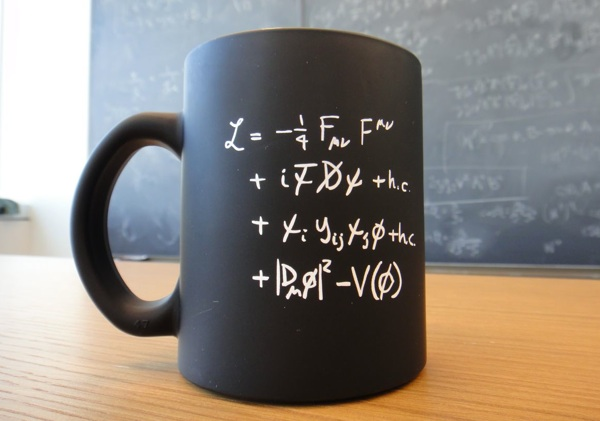
\includegraphics[width=\textwidth]{slides/figures/cernmug.jpeg}
        \column{0.5\textwidth}
        \begin{itemize} 
            \item The Standard Model (SM) represents the our current best understanding of the matter and force.
            \item It includes three generations of leptons (\Pe\PGne), (\PGm\PGnGm), (\PGt\PGnGt) and quarks (\PQu\PQd), (\PQc\PQs), (\PQt\PQb) as matter paticles, four gauge bosons \PGg, \PW, \PZ, \Pg as force particles, and one Higgs boson to generate mass.
            \item SM has been very successful in explaining and predicting experimental observations so far.
        \end{itemize}
    \end{columns}
    
    \vspace{0.05\textheight}
    \begin{itemize}
        \item The interaction between the leptons and \PW boson is encapsulated in the term $i\bar{\psi}\slashed{D}\psi$:
        \begin{equation*} \tiny
            i\bar{\psi}\slashed{D}\psi = 
            \bar{\chi}_L \gamma^\mu \big( i \partial_\mu  - \textcolor{red}{g} \frac{\tau_a}{2} W^a_\mu  -g'\frac{Y}{2} B_\mu \big) \chi_L 
            + \bar{\psi}_R \gamma^\mu \big( i \partial_\mu -g'\frac{Y}{2} B_\mu \big) \psi_R 
            - g_s (\bar{q}\gamma^\mu  T_{a} q) G_\mu^a 
        \end{equation*}
    \end{itemize}
\end{frame}



% -------------
% new frame
% -------------
\begin{frame}{Introduction}
\smaller 
    
    \begin{center}
    \resizebox{0.6\textwidth}{!}{    \feynmandiagram [inline=(d.base), small, horizontal=d to b] {
        a[particle=\PGne] -- [fermion] b [dot] -- [fermion] c[particle=\Pe], 
        b -- [boson, edge label=\PW] d,}; 
    = \qquad
    \feynmandiagram [inline=(d.base), small, horizontal=d to b] {
        a[particle=\PGnGm] -- [fermion] b [dot] -- [fermion] c[particle=\PGm],
        b -- [boson, edge label=\PW] d, }; 
    = \qquad
    \feynmandiagram [inline=(d.base), small, horizontal=d to b] {
        a[particle=\PGnGt] -- [fermion] b [dot] -- [fermion] c[particle=\PGt],
        b -- [boson, edge label=\PW] d,};}
    \end{center}
    
    \vspace{0.05\textheight}
    \begin{itemize} 
        \item One of the essential assumptions in SM is that the coupling strength $g$ is the same for all three generations of leptons, $g_\Pe = g_\PGm = g_\PGt \equiv g $, known as Lepton Universality (LU) in the weak interaction.
        \item Tests of the SM LU can be performed by studies of the leptonic decays of \PW bosons.
        \item In high-energy regime, the tests of lepton universality related to \PW boson have been performed on colliders.
        \begin{itemize} 
        \smaller 
            \item SPS and Tevatron using $\Pp\bar{\Pp}\to \PW$.
            \item LEP using $\Pe\bar{\Pe}\to \PW \PW$.
            \item LHC using $\Pp\Pp \to \PW$ and $\Pp\Pp \to \ttbar \to \PQb\PW \PAQb\PW$.
        \end{itemize}
        \item In low-energy regime, some of the most stringent LU tests come from the charge weak decays of mesons (e.g. \PD, \PB) and leptonic decays of taus \cite{Amhis:2019ckw}. While most show high precision agreement with LU, tensions have been recently observed in the semileptonic decays of \PB mesons by Belle \cite{Huschle:2015rga, Sato:2016svk, Hirose:2016wfn}, BaBar  \cite{Lees:2012xj, Lees:2013uzd} and LHCb \cite{Aaij:2015yra,Aaij:2017uff, Aaij:2017deq}.
    \end{itemize}
\end{frame}



% -------------
% new frame
% -------------
\begin{frame}{}
\smaller
    
    \begin{block}{SPS and Tevatron}
        \begin{columns}
            % add column
            \column{0.65\textwidth}
            \begin{itemize}
                \item the $\sigma_{\Pp\bar{\Pp}\to \PW} \times \BWl$ in three leptonic channels were measured by UA1 \cite{Albajar:1988ka}, UA2 \cite{appel1986measurement, Alitti:1991eh, Alitti:1992hv}, CDF \cite{Abe:1990sd, Abe:1992ys, Abe:1991fb}, D0 \cite{Abbott:1999tt, Abazov:2003sv, Abachi:1995xc, Abbott:1999pk}.
                \item taus were reconstructed in the hadronic decay modes.
                \item Combined average $g^\PW_\PGt / g^\PW_\Pe = 0.988\pm 0.025$ were determined by \DZERO \cite{Abbott:1999pk} consistent with SM.  
            \end{itemize}
            
            % add column
            \column{0.3\textwidth}
            \centering
            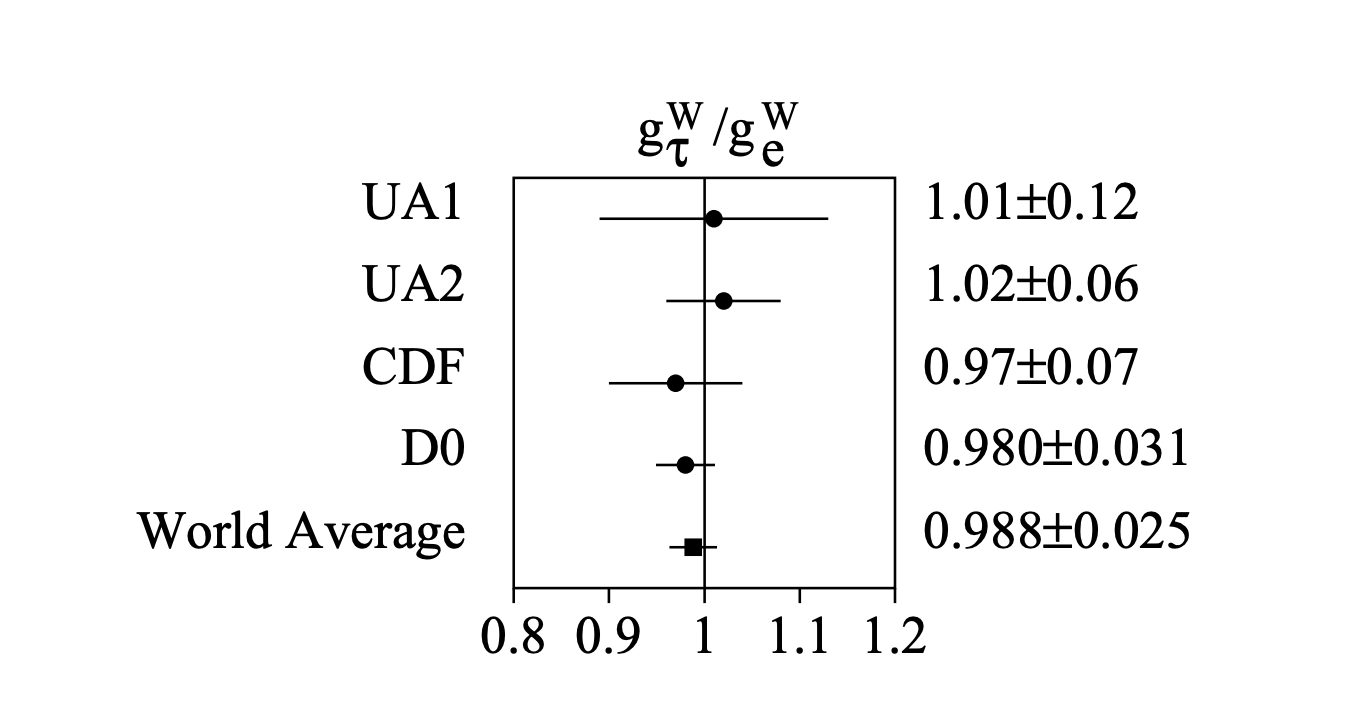
\includegraphics[width=\textwidth]{chapters/Introduction/sectionRelatedWorks/figures/spsTevatron.png}
        \end{columns}
    \end{block}
    
    \begin{block}{LEP-II}
        \begin{columns}
            % add column
            \column{0.65\textwidth}
            \begin{itemize}
                \item three individual leptonic \BWl were measured using pair-produced \WW from the electron-position collision by OPAL \cite{Abbiendi:2007rs}, DELPHI \cite{Abdallah:2003zm}, L3 \cite{Achard:2004zw}, ALEPH \cite{Heister:2004wr}.
                \item the most precise and the only \BWl measurement available in PDG~\cite{pdg2020}.
                \item The LEP combined result \cite{Schael:2013ita} showed agreement between electron and muon channel agree with each other, but tau channel was $2.6 \; \sigma$ above the average $$ \tiny \frac{2\times\BWt}{\BWe+\BWm} = 1.066 \pm 0.025 $$ comparing with the SM prediction 0.999 \cite{Denner:1991kt,Rtau,dEnterria:2016rbf}.
            \end{itemize}
            
            % add column
            \column{0.3\textwidth}
            \centering
            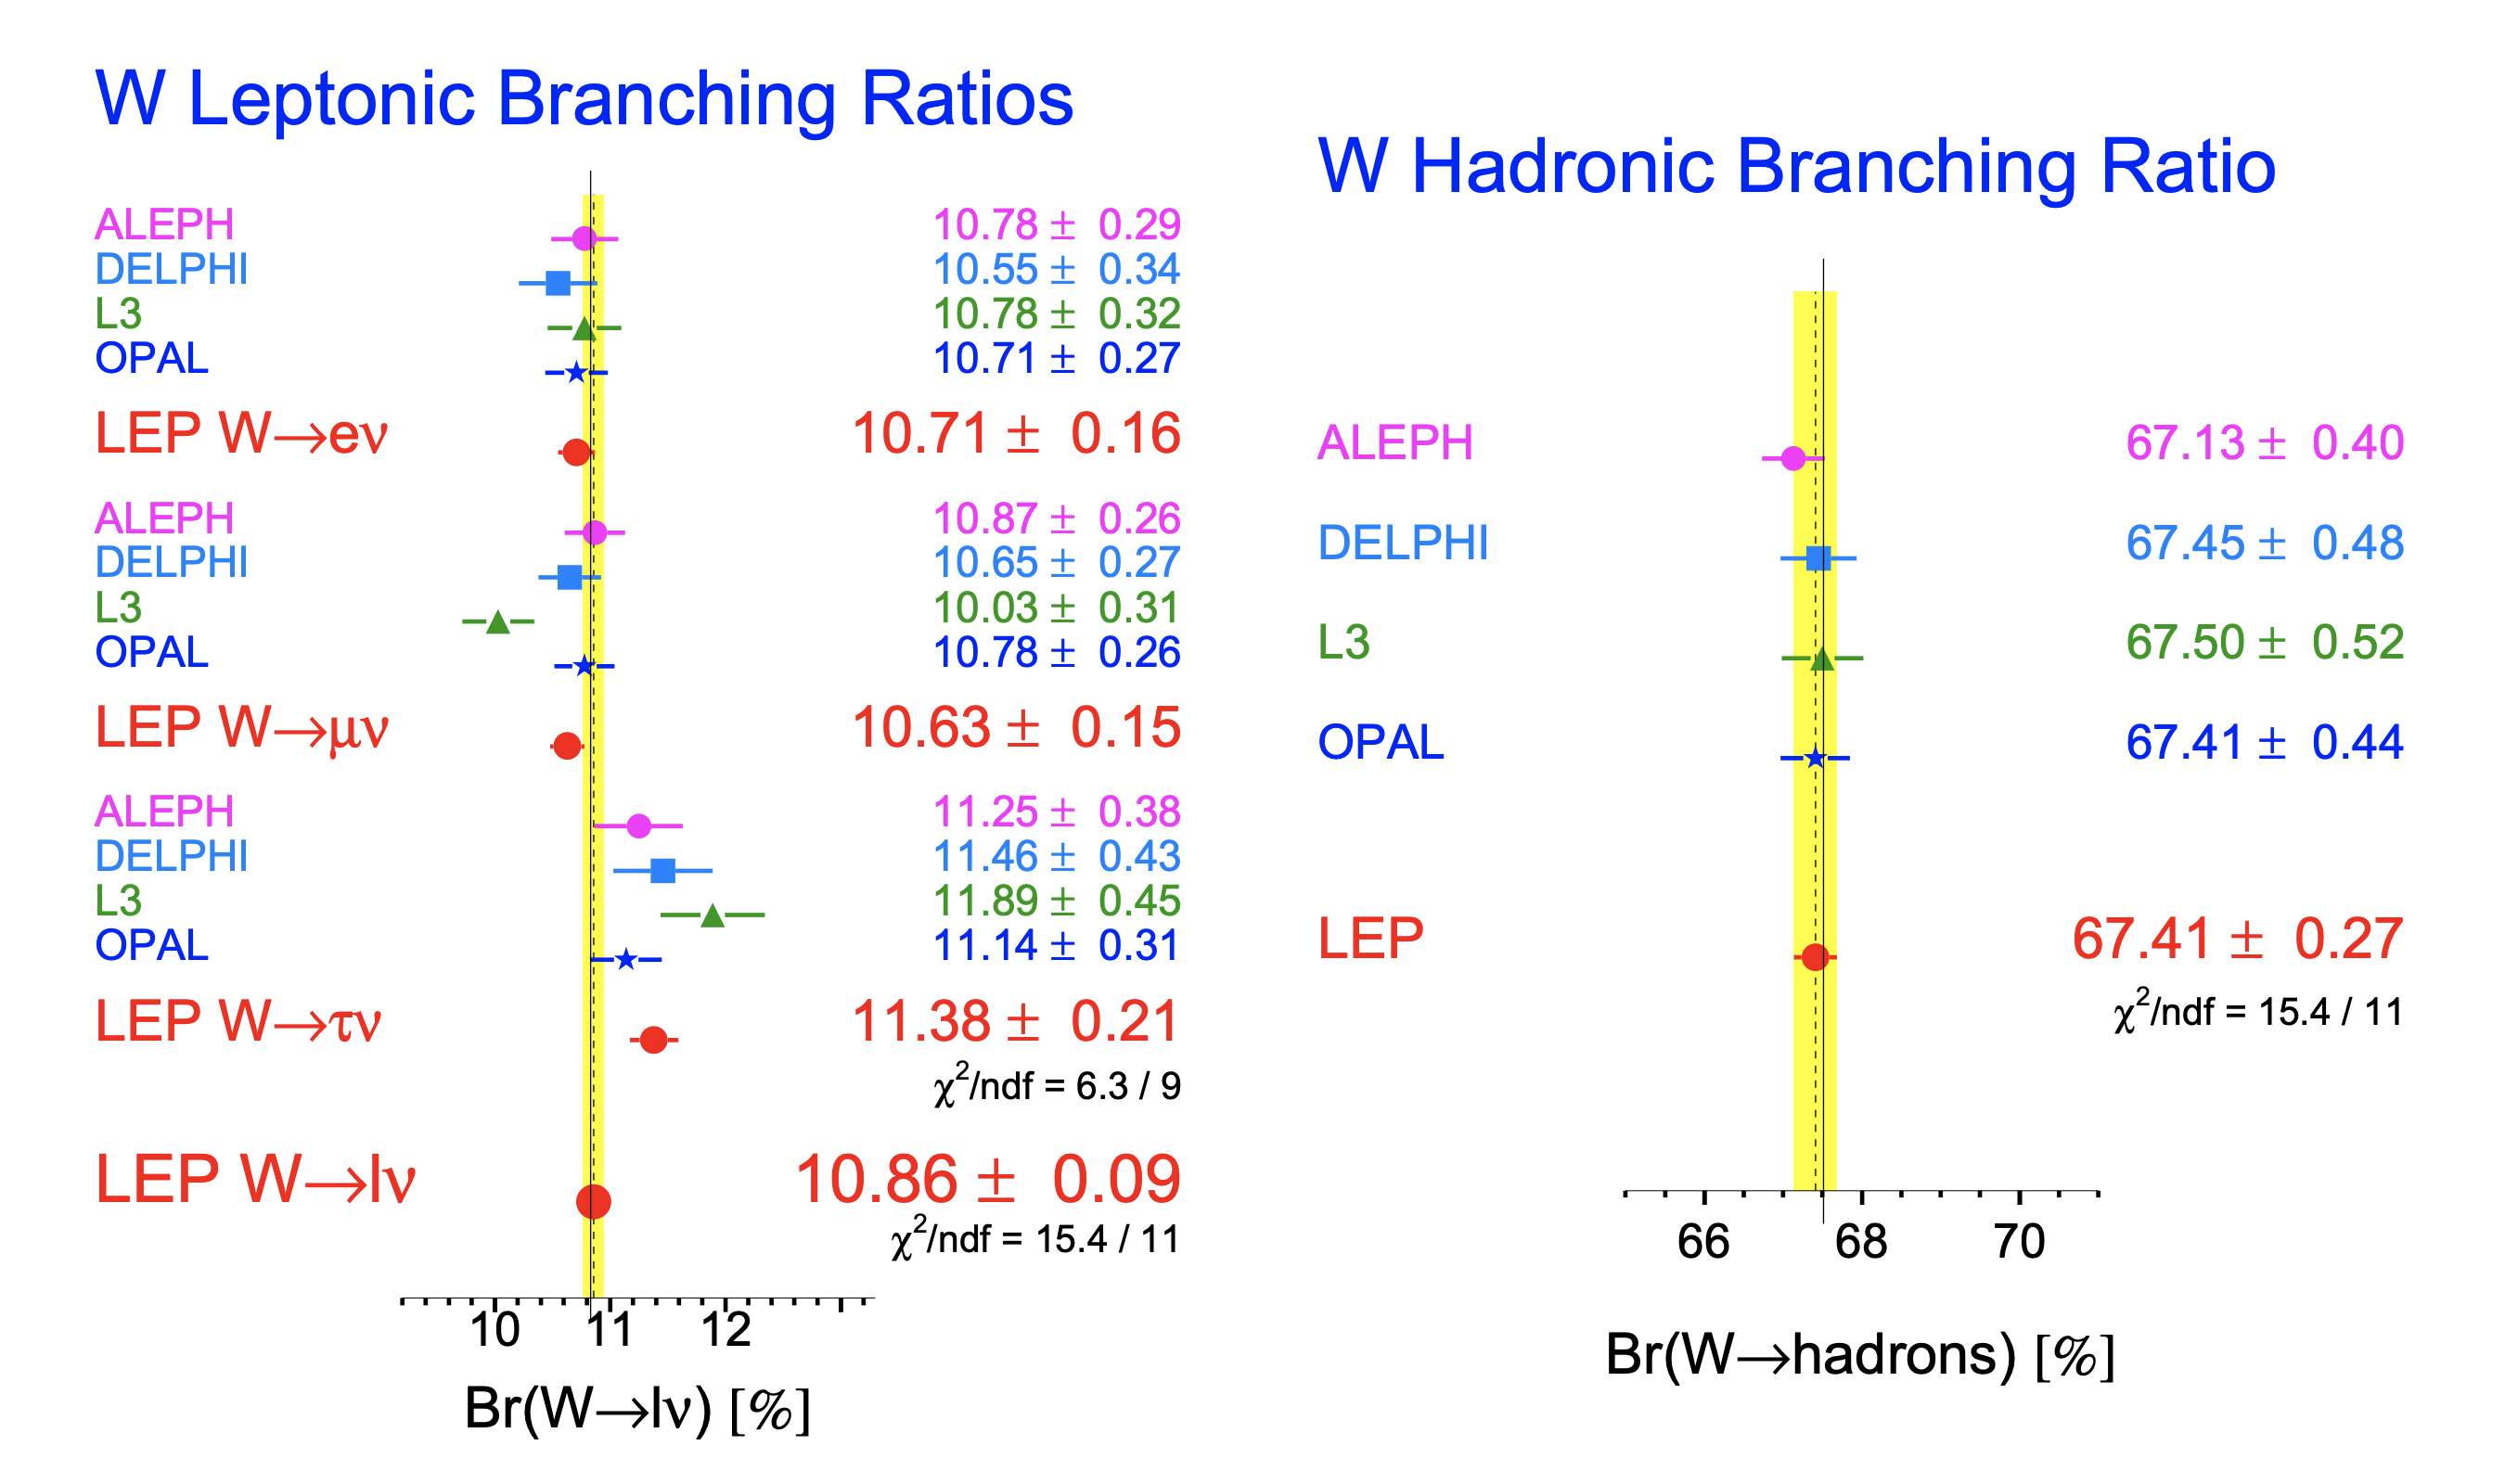
\includegraphics[width=\textwidth, trim=0 0 25cm 0, clip]{chapters/Introduction/sectionRelatedWorks/figures/lep.png}
        \end{columns}
    \end{block}
\end{frame}





% -------------
% new frame
% -------------
\begin{frame}{}
\smaller
    
    \begin{block}{LHC run-1}
        In the LHC run-1 at $\sqrt{s}=$ 7\TeV and 8\TeV, the LU between $\PW \to \Pe \PGn$ and $\PW \to \PGm \PGn$ has been tested by ATLAS \cite{Aaboud:2016btc} and LHCb \cite{Aaij:2015zlq, Aaij:2016qqz}.
        \begin{itemize}
            \item the \wjets cross-section was measured in electron and muon channels, ratio of which leads to $\BWm/\BWe$ as 1.003(10) by ATLAS and 0.980(18) by LHCb.
            \item the results agree with SM lepton universality.
        \end{itemize}
    \end{block}
                
   \begin{block}{LHC run-2}
        \begin{columns}[c]
            % add column
            \column{0.65\textwidth}           
            In the LHC run-2 at $\sqrt{s}=$ 13\TeV, ATLAS \cite{Aad:2020ayz} has most recently published a test between muon and tau.
            \begin{itemize}
                \item use $\Pp\Pp\to\ttbar\to\PQb\PW\PAQb\PW$ events selected with \cmm, \cem plus two \PQb tagged jets final states.
                \item tau leptons are probed via muons from $\PGt\to\PGm\PAGnGm\PGnGt$, which tend to be softer and more displaced than prompt muons.
                \item fitting the transverse displacement and \pt of the probing muon leads to the ratio $$ \tiny \BWt/\BWm = 0.992 \pm 0.013 $$ consistent with the LU.
            \end{itemize}
            
            % add column
            \column{0.3\textwidth}
            \centering
            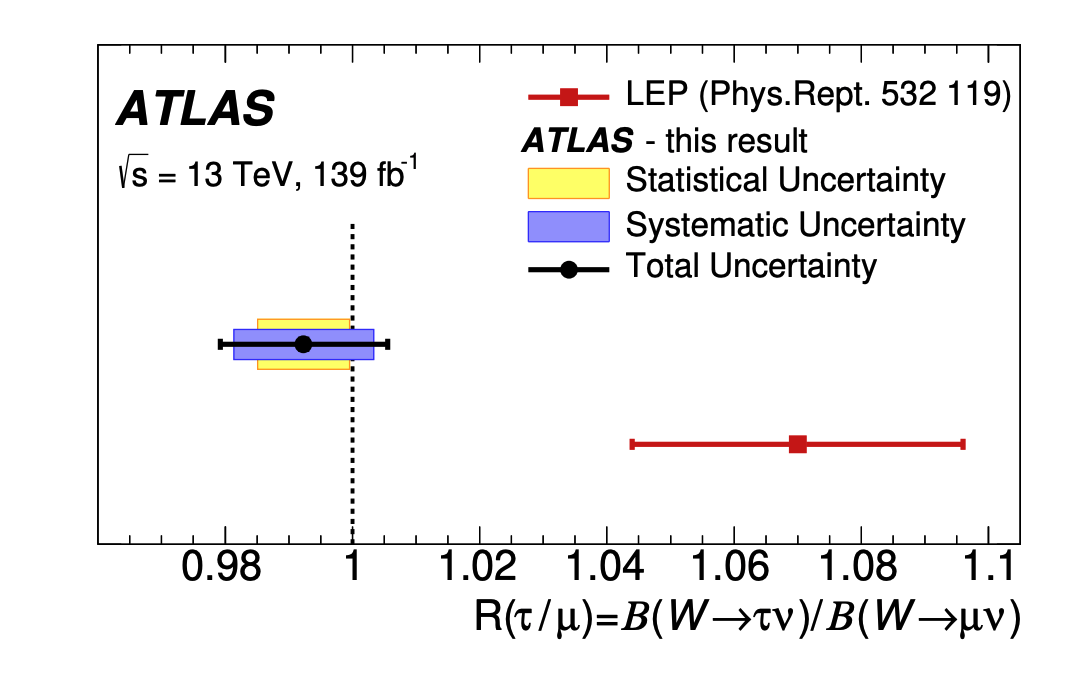
\includegraphics[width=\textwidth]{chapters/Introduction/sectionRelatedWorks/figures/atlas.png}
        \end{columns}
    \end{block}
\end{frame}






% -------------
% new frame
% -------------
\begin{frame}{}
\smaller
    \begin{columns}
        % add column
        \column{0.55\textwidth}
        \begin{block}{}
            \centering
            \small{\ttbar} process
            \resizebox{0.98\textwidth}{!}{    \feynmandiagram[small,horizontal=a to b]{
        i1 [particle=\PQq] -- [fermion] a -- [fermion] i2 [particle=\PQq],
        a -- [gluon, edge label=\Pg] b,
        f1 [particle=\PQt] -- [fermion] b -- [fermion] f2 [particle=\PQt],
        % top decay
        f1b[particle=\PQb] -- [fermion] f1 -- [photon] f1W [particle=\PW, red],
        f2b[particle=\PQb] -- [anti fermion] f2 -- [photon] f2W [particle=\PW, red],
        f1 -- [opacity=0.0] f2,
        f1W -- [opacity=0.0] f2W,
        f1b -- [opacity=0.0] f1W,
        f2b -- [opacity=0.0] f2W,
    }; \qquad
    \feynmandiagram[small,horizontal=a to b]{
        i1 [particle=\Pg] -- [gluon] a -- [gluon] i2 [particle=\Pg],
        a -- [gluon, edge label=\Pg] b,
        f1 [particle=\PQt] -- [fermion] b -- [fermion] f2 [particle=\PQt],
        % top decay
        f1b[particle=\PQb] -- [fermion] f1 -- [photon] f1W [particle=\PW, red],
        f2b[particle=\PQb] -- [anti fermion] f2 -- [photon] f2W [particle=\PW, red],
        f1 -- [opacity=0.0] f2,
        f1W -- [opacity=0.0] f2W,
        f1b -- [opacity=0.0] f1W,
        f2b -- [opacity=0.0] f2W,
    }; \qquad
    \feynmandiagram[small, vertical=a to b, horizontal=a to f1]{
        i1 [particle=\Pg] -- [gluon] a -- [anti fermion] f1 [particle=\PQt],
        a -- [fermion, edge label=\PQt] b,
        i2 [particle=\Pg] -- [gluon] b -- [fermion] f2 [particle=\PQt],
        % top decay
        f1b[particle=\PQb] -- [fermion] f1 -- [photon] f1W [particle=\PW, red],
        f2b[particle=\PQb] -- [anti fermion] f2 -- [photon] f2W [particle=\PW, red],
        f1 -- [opacity=0.0] f2,
        f1W -- [opacity=0.0] f2W,
        f1b -- [opacity=0.0] f1W,
        f2b -- [opacity=0.0] f2W,
        % i1 -- [opacity=0.0] i2,
        % f1 -- [opacity=0.0] f2,
    };}
        \end{block}
        % add column
        \column{0.4\textwidth}
        \begin{block}{}
            \centering
            \small{\tW} process
            \resizebox{0.98\textwidth}{!}{    \feynmandiagram[scale=0.7][horizontal=a to b]{
        i1 [particle=\PQb] -- [fermion] a -- [gluon] i2 [particle=\Pg],
        a -- [fermion, edge label=\PQb] b,
        f1 [particle=\PW , red] -- [photon] b -- [fermion] f2 [particle=\PQt],
        f2b[particle=\PQb] -- [anti fermion] f2 -- [photon] f2W [particle=\PW, red],
        f1 -- [opacity=0.0] f2W,
    }; \qquad
    \feynmandiagram[scale=0.7][vertical=a to b]{
        i1 [particle=\PQb] -- [fermion] a -- [photon] f1 [particle=\PW, red],
        a -- [fermion, edge label=\PQb] b,
        i2 [particle=\Pg] -- [gluon] b -- [fermion] f2 [particle=\PQt],
        f2b[particle=\PQb] -- [anti fermion] f2 -- [photon] f2W [particle=\PW, red],
        i1 -- [opacity=0.0] i2,
        f1 -- [opacity=0.0] f2W -- [opacity=0.0] f2b,
    };}
        \end{block}
    \end{columns}
    
    \vspace{0.1\textheight}
    \begin{itemize}
        \item This analysis presents a CMS measurement of three individual \BWl and a test of lepton universality in the \PW decay, 
        \begin{itemize} 
        \smaller
            \item use the run 2016 dataset from the LHC $\sqrt{s}=13\TeV$ proton-proton collisions.
            \item treat \ttbar and \tW processes as the primary signals.
        \end{itemize}       
        \item Motivations
        \begin{itemize} 
        \smaller
            \item The measurements of three \PW leptonic branching fractions have not been improved for more than a decay since LEP;
            \item LEP's $R_{\PGt/(e,\PGm)}$ shows a $2.6\,\sigma$ deviation from the SM prediction.
        \end{itemize}
        \item Opportunities
        \begin{itemize} 
        \smaller
            \item LHC 13\TeV \Pp-\Pp collisions produce a large number of \ttbar events giving $\PW\PW$ pairs;
            \item The improved \PQb tagging allows to select \ttbar events with a high purity;
            \item The improved \PGth identification enables to efficiently select \PW tauonic decays.
        \end{itemize}
    \end{itemize}
\end{frame}
    
    
    
    
    
% \begin{frame}{Introduction}
%     \begin{center}
%     \begin{itemize} \smaller
%         \item A
%         \item B
%     \end{itemize}
%     \end{center}
    
%     \begin{center}
%     \begin{columns}
%         % add column
%         \column{0.4\textwidth}
%         add column
        
%         % add column
%         \column{0.6\textwidth}
%         add column
%     \end{columns}
%     \end{center}
% \end{frame}
    

            

        

